\documentclass[12pt]{article}

% Package Imports
\usepackage{amsmath,amssymb}  % Math symbols
\usepackage{graphicx}         % For figures
\usepackage[margin=1in]{geometry}  % Standard margin
\usepackage{setspace}         % Adjust line spacing
\usepackage{authblk}          % For authors and affiliations
\usepackage{caption}          % For figure captions
\usepackage{subfigure} 
\usepackage[numbers, sort]{natbib} % 保证参考文献不会出现乱序

% Title and Author Setup
\title{quantms, ms2rescore and multiple search engines enables deep proteome coverage across protein quantification, immunopeptidomics, and phosphoproteomics experiments}
\author[1,2]{Chengxin Dai}
\author[3,4]{Ralf Gabriels}
\author[3,4]{Robbin Bouwmeester}
\author[5,6,7,8]{Jonas Scheid}
\author[3,4,9,10]{Lennart Martens}
\author[12]{Oliver Kohlbacher}
\author[11]{Mingze Bai}
\author[12]{Timo Sachsenberg}
\author[13]{Yasset Perez-Riverol\thanks{Corresponding author: yperez@ebi.ac.uk}}
\affil[1]{State Key Laboratory of Medical Proteomics, Beijing Proteome Research Center, National Center for Protein Sciences (Beijing), Beijing Institute of Lifeomics, 102206, Beijing, China}
\affil[2]{International Academy of Phronesis Medicine (Guangdong), 510320, Guangdong, China}
\affil[3]{VIB Center for Medical Biotechnology, VIB, Ghent, 9052, Belgium}
\affil[4]{Department of Biomolecular Medicine, Faculty of Medicine and Health Sciences, Ghent University, Ghent, 9052, Belgium}
\affil[5]{Department of Peptide-based Immunotherapy, Institute of Immunology, University and University Hospital Tübingen, Tübingen, Germany}
\affil[6]{Cluster of Excellence iFIT (EXC2180) "Image-Guided and Functionally Instructed Tumor Therapies", University of Tübingen, Tübingen, Germany}
\affil[7]{Quantitative Biology Center (QBiC), University of Tübingen, Tübingen, Germany}
\affil[8]{Institute for Bioinformatics and Medical Informatics (IBMI), University of Tübingen, Tübingen, Germany}
\affil[9]{BioOrganic Mass Spectrometry Laboratory (LSMBO), IPHC UMR 7178, University of Strasbourg, CNRS, Strasbourg, 67000, France}
\affil[10]{Infrastructure Nationale de Proteomique ProFI - FR2048, Strasbourg, 67087, France}
\affil[11]{Chongqing Key Laboratory of Big Data for Bio Intelligence, Chongqing University of Posts and Telecommunications, Chongqing, China}
\affil[12]{Department of Computer Science, Applied Bioinformatics, University of Tübingen, Tübingen, Germany}
\affil[13]{European Molecular Biology Laboratory, European Bioinformatics Institute, Wellcome Genome Campus, Cambridge, United Kingdom}
\date{}

% Document Begins
\begin{document}
\maketitle
\doublespacing  % MCP requires double-spacing

% Abstract Section
\begin{abstract}
The exponential growth of public proteomics datasets has surpassed the analytical capacity of traditional desktop tools, particularly for large-scale automated reanalysis. To address this challenge, we present an integrated workflow that combines quantms, a cloud-native pipeline, with MS²Rescore, a machine learning-based rescoring tool. This workflow enables deep and scalable reanalysis of massive proteomic datasets. Powered by the Nextflow engine for parallel computing, the pipeline incorporates fragment ion intensity predictions from MS²PIP and retention time predictions from DeepLC, improving peptide-spectrum match reliability through Percolator. We applied this approach to four representative datasets covering label-free quantification, TMT labeling, immunopeptidomics, and phosphoproteomics. Compared to traditional methods, our workflow achieved a 16–22.8\% increase in identified spectra, along with the quantification of hundreds of additional proteins and phosphosites. These improvements demonstrate that integrating multiple search engines with machine learning-derived features not only enhances identification sensitivity but also deepens quantitative insights for downstream biological interpretation. Overall, this workflow offers a reproducible and scalable solution for the reanalysis of public proteomics data, advancing FAIR principles by promoting scientific transparency, accessibility, and data reuse.

\end{abstract}

% Keywords
\noindent\textbf{Keywords:} Proteomics, Reanalysis, Workflow, Machine learning.

% Main Content
\section{Introduction}
In recent years, the field of proteomics has experienced rapid growth in the availability of publicly accessible datasets, accompanied by a shift toward studies analyzing larger sample cohorts. As of June 2025, over 40,000 datasets have been submitted to ProteomeXchange (PX) repositories, including a substantial increase in large-scale submissions comprising more than 100 instrument files \cite{perez-riverol_pride_2025}. However, conventional desktop tools such as MaxQuant \cite{cox_maxquant_2008}, pFind \cite{wang_pfind_2007}, PeptideShaker \cite{vaudel2015peptideshaker}, and Proteome Discoverer are limited in their capacity to perform automated, large-scale quantitative analyses in cloud or distributed environments, hindering the reanalysis of extensive experiments on standard workstations. % to be fair, there are ways to call some of these tools from the command line or on server infrastructure, right? If you look at spectronaut currently they are also making a big push towards cloud computing. Proteome discoverer offers services to be offloaded to other servers too I believe.

We recently developed quantms \cite{dai_quantms_2024}, an open-source, cloud-based pipeline designed for massively parallel reanalysis of quantitative proteomic datasets. The pipeline is highly modular and flexible, accommodating a wide range of quantitative proteomics approaches including DDA label-free, DDA multiplex (TMT and ITRAQ) and DIA. % Consider to oxford comma ", DDA multiplex (TMT and ITRAQ), and DIA."
quantms automatically distributes computations using the Nextflow workflow engine across one or more computing nodes, depending on the number of instrument files and samples \cite{di_tommaso_nextflow_2017}. To ensure traceability and reproducibility, the pipeline is built entirely on standardised open file formats and reproducible execution environments, adhering strictly to the FAIR (Findability, Accessibility, Interoperability, and Reusability) principles \cite{wilkinson_fair_2016}. quantms has been extensively benchmarked and used in the analysis of large-scale public proteomics datasets \cite{dai_quantms_2024,bai2023lfq, ZHENG2025105440}.

To address this limitation, we recently developed quantms, an open-source, cloud-based pipeline designed for massively parallel reanalysis of quantitative proteomic datasets \cite{dai_quantms_2024}. The pipeline is highly modular and flexible, accommodating a wide range of quantitative proteomics approaches. quantms automatically distributes computations using the Nextflow workflow engine across one or more computing nodes, depending on the number of instrument files and samples \cite{di_tommaso_nextflow_2017}. To ensure traceability and reproducibility, the pipeline is built entirely on standardized open file formats and reproducible execution environments \cite{dai_proteomics_2021} \cite{martens_mzmlcommunity_2011}, adhering strictly to the FAIR (Findability, Accessibility, Interoperability, and Reusability) principles \cite{wilkinson_fair_2016}.

With the integration of machine learning (ML) into proteomics, various models have been developed to accurately predict peptide behavior in LC-MS, such as MS²PIP \cite{degroeve_ms2pip_2013} and DeepLC \cite{bouwmeester_deeplc_2021} for fragment ion intensities and retention time prediction, respectively. Early approaches employed decision trees and single-layer neural networks, while more recent deep learning models such as Prosit \cite{gessulat_prosit_2019} achieve significantly improved accuracy for predicting fragment ion intensities and retention times. These highly accurate predictions enable superior matching of experimental data to theoretical expectations and have reinvigorated rescoring strategies in proteomics. % Ok, but MS²Rescore is still using MS2PIP which is classical ML
MS²Rescore represents a modular package that generates multiple features assessing the similarity between observed and predicted MS/MS spectra utilizing MS²PIP. Furthermore, MS²Rescore calculates RT-dependent features, e.g., delta RT, utilizing DeepLC \cite{buur_ms2_2024}.

Previously, quantms did not leverage measurable peptide properties such as fragment ion intensities and retention times. To overcome this limitation, we integrated MS²Rescore into quantms and incorporated customized features following Nextflow and nf-core best practices. We demonstrate that the enhanced pipeline supports in-depth analysis of large-scale public proteomics datasets across diverse experimental designs, including label-free quantification (LFQ), tandem mass tag (TMT)-based quantification, immunopeptidomics, and phosphoproteomics studies.

\section{Methods}

\subsection{MS/MS Data and quantms Search Results}
To develop and evaluate the performance of the quantms-integrated MS²Rescore workflow, we selected four publicly available benchmark datasets. Three were obtained from the PRIDE Archive under the identifiers PXD001819, PXD019643, and PXD026824, and one from the CPTAC data portal under PDC000127. The PXD001819 dataset contains 48 Sigma UPS1 proteins spiked into a background of yeast cell lysate at nine different concentrations: 0.05, 0.125, 0.25, 0.5, 2.5, 5, 12.5, 25, and 50 fmol/$\mu$L to evaluate quantification performance. We evaluated five different quantms workflow settings: (1) Comet, (2) Comet and MSGF+, (3) Comet with MS²Rescore, (4) Comet and MSGF+ with MS²Rescore, and (5) Comet, MSGF+, and SAGE with MS²Rescore to explore multiple search engines and their integration with MS²Rescore for improved identification and quantification results. All search parameters were the same as described in the previous publication. An FDR filter at 1\% was applied at peptide spectrum match (PSM) and protein level at the dataset level. The search results from quantms and MaxQuant at the PSM and protein group levels are provided in Supplemental File S1.

\subsection{Rescoring Features and Postprocessing}
 The quantms-rescoring Python package integrates MS²Rescore and computes a broad range of features based on DeepLC-predicted versus observed retention times, as well as MS²PIP-predicted versus observed MS2 fragment ion intensities. Signal-to-noise ratio (SNR) features are also computed for specific scenarios. % This part is not entirely clear to me.
 To enhance compatibility and performance, we implements new strategies for model selection, feature export, and model training. For retention time (RT)-related features, retraining of the DeepLC model is supported, allowing the selection of the model with the lowest mean absolute error (MAE) on calibration PSMs. These calibration PSMs are selected from each run at a specified ratio. % We can now cite: https://www.biorxiv.org/content/10.1101/2025.06.01.657225v1.full
 For MS2 intensity-related features, we perform overfitting tests using the top-scoring 60\% of non-decoy PSMs in the calibration set. quantms-rescoring automatically selects the most suitable MS²PIP model for a given batch of PSMs by comparing the correlation scores of predicted and observed intensities across candidate models. Furthermore, it verifies whether the MS²PIP predictions meet predefined correlation and scoring thresholds. This is achieved by filtering out decoy PSMs, ranking the results by PSM score, and selecting a calibration subset. The method ensures that at least 80\% of calibration PSMs exceed the correlation threshold. If none of the models satisfy this criterion, MS²PIP rescoring is skipped unless explicitly forced by the user. This mechanism prevents the use of poorly fitting models and filters out pre-trained models that are incompatible with the data. Additionally, users can specify a list of features for export. All steps are fully parallelized at the run level, significantly reducing runtime for large-scale datasets.
 
 Then, the quantms workflow calculates a posterior error probability for each PSM using Percolator. This is performed under three different feature configurations (1) a baseline model using only search engine-derived features, (2) the baseline model plus MS²Rescore-derived features, and (3) the above combined with SNR features. To merge results from multiple search engines, ConsensusID aggregates PSMs into unified scores. Final PSM-level q-values are then obtained either directly from Percolator or calculated using OpenMS' target-decoy approach based on the predicted probabilities. For phosphoproteomics datasets, LuciPHOr2 is employed to assign site-level localization scores and estimate the associated false localization rate using tools from the OpenMS toolkit. % cite openms; https://www.nature.com/articles/nmeth.3959

\section{Results}

\subsection{quantms with MS²Rescore Enhances Label-Free Identification and Quantification}
To systematically evaluate the performance of the quantms-integrated MS²Rescore workflow at both identification and quantification levels, we first analyzed the public benchmark dataset PXD001819. For benchmarking the identifications, five different workflows configurations were designed and compared, including (1) Comet with Percolator, (2) two search engines with Percolator, (3) Comet with MS²Rescore features and Percolator, (4) two search engines with MS²Rescore features and Percolator, and (5) three search engines with MS²Rescore features and Percolator to determine whether features from intensity-based and retention time-based predictors enhanced the identification and quantification process. % enhanced is maybe a bit vague, improve sensitivity and/or specificity of identifications and quantifications?

Significant PSMs were filtered based on q-values, and the FDR was used as a key metric to compare workflows. As shown in Figure ~\ref{fig:PXD001819_ms2rescore_pic}, using consensus scores from two search engines significantly increased identification rates at a fixed FDR threshold. Specifically, combining Comet and MSGF+ improved identified spectra by 17\% over Comet alone, and incorporating MS²PIP and DeepLC features through MS²Rescore led to an additional 16\% increase. quantms achieved a 28\% improvement in the number of PSM identifications compared to MaxQuant. At the quantification level, including MS²Rescore-derived features allowed more low-abundance UPS1 proteins to be quantified (Figure 2B), highlighting the contributions of the integrated workflow. Although MaxQaunt reported more UPS proteins in 2500amol, the proteins that were only quantified in MaxQuant were all quantified by match between runs (MBR) rather than from MS/MS. The main reason for this is that quantms used different MBR quality control.

To better understand the contribution of individual features, we extracted the top 20 feature weights from Percolator (Supplemental Figure 1). Over half of the top-weighted features were derived from MS²Rescore. Notably, SpecPearsonNorm had a strong positive weight, indicating that a better correlation between predicted and observed intensities improves confidence. Conversely, RtDiffBest had a negative weight, suggesting that large deviations in retention time reduce match quality. Interestingly, peptide length also emerged as a significant positive feature after MS²Rescore integration, likely because longer peptides generate more fragment ions and thus are more reliably identified.

% Figure Example
\begin{figure}[ht!]
	\centering
	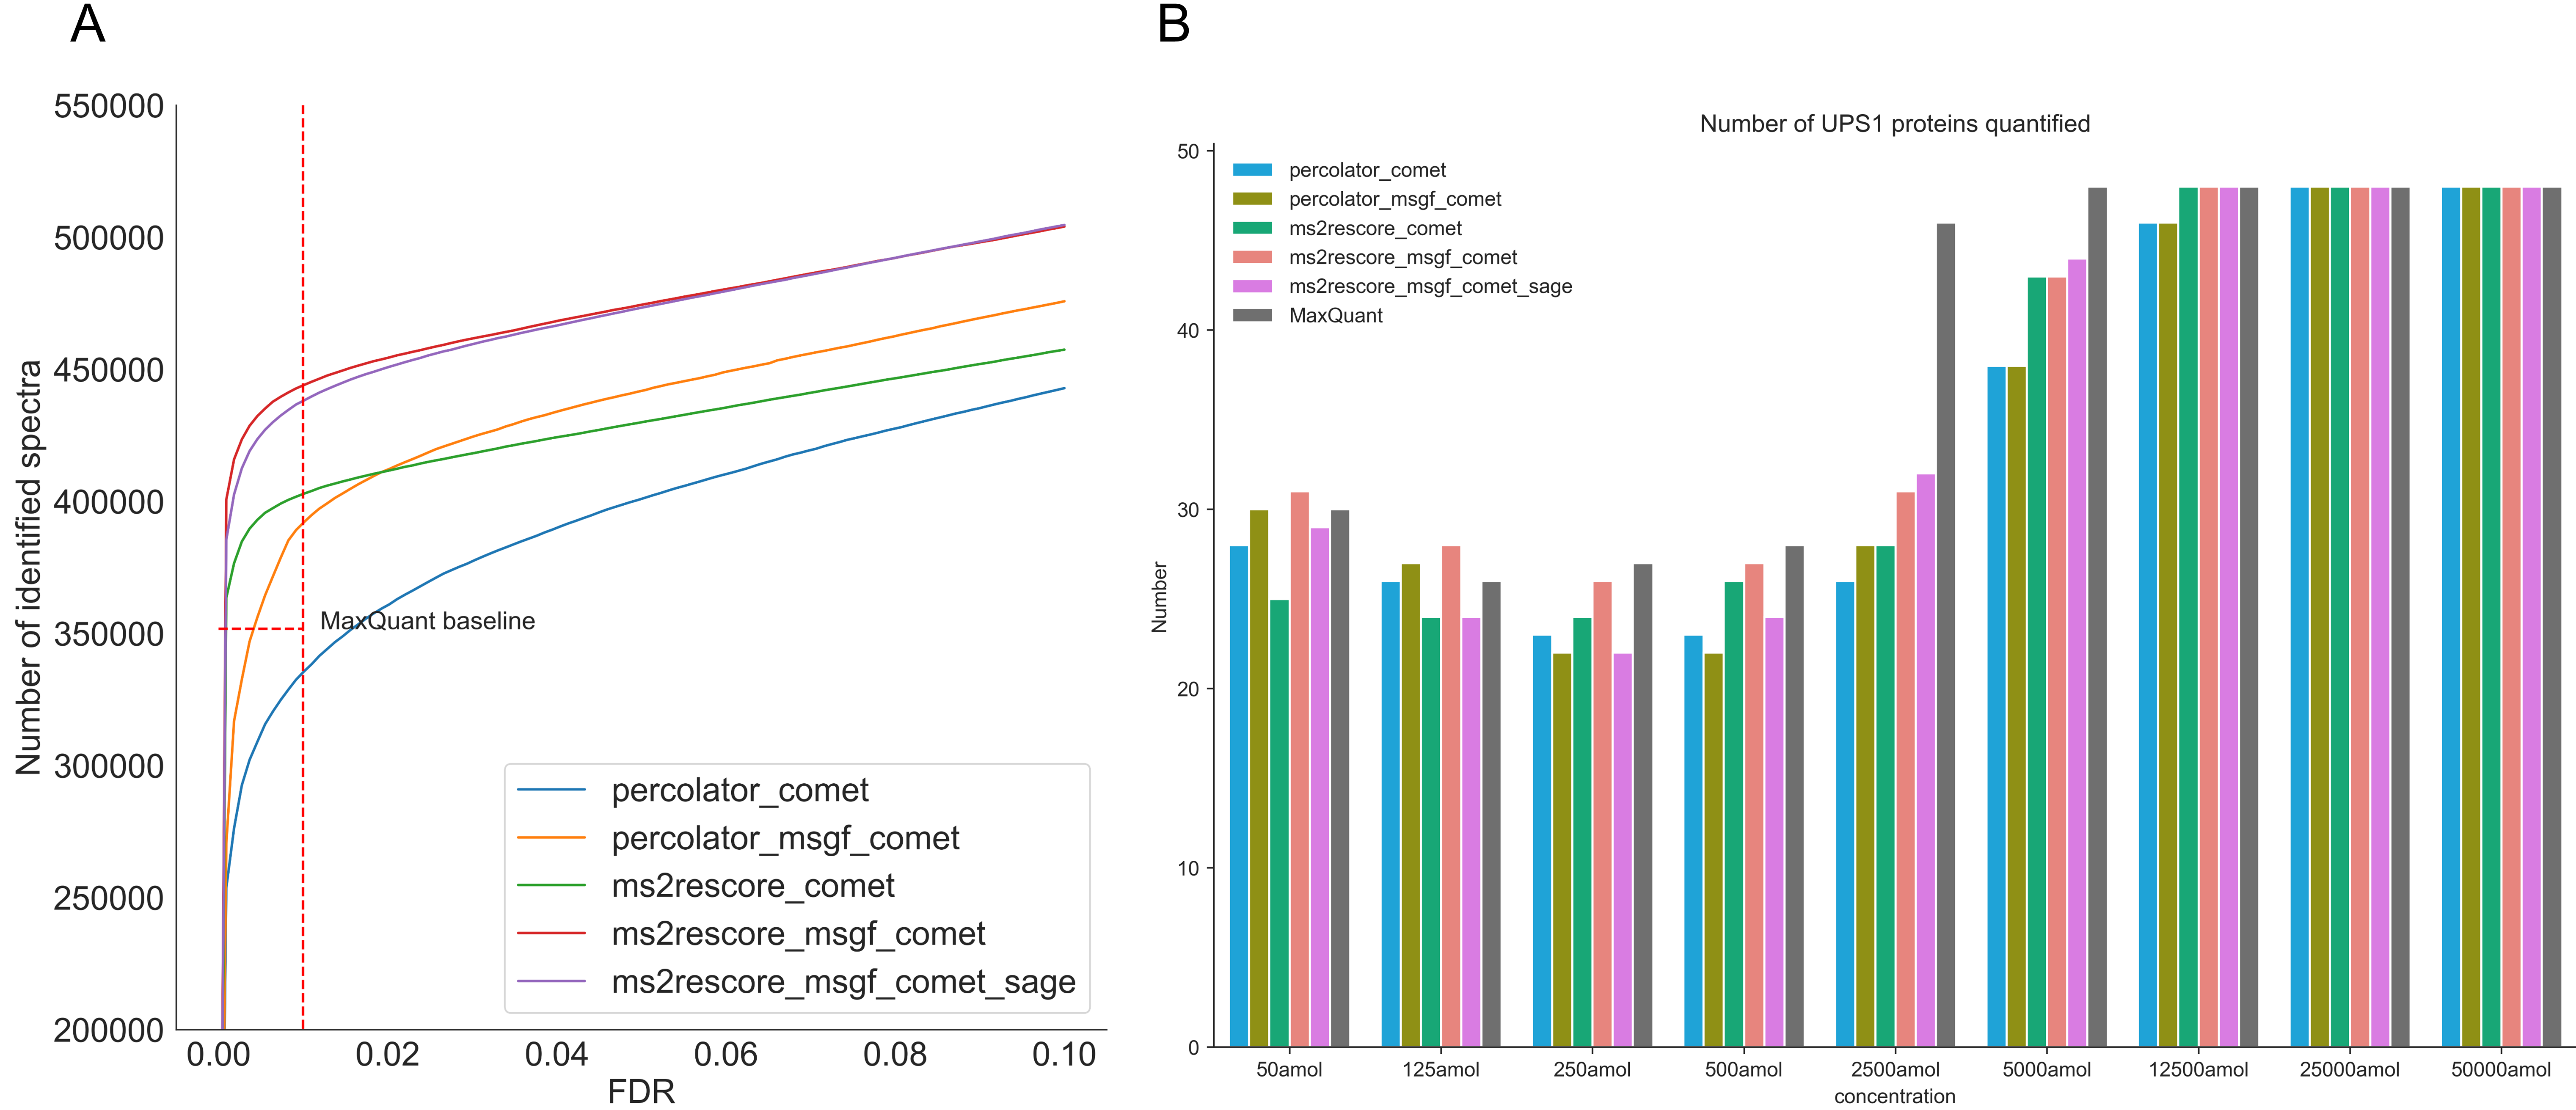
\includegraphics[width=1\textwidth]{figures//PXD001819.png}
	\caption{The number of identified spectra as a function of differing FDR levels for different workflow settings. (A) Results for the PXD001819 dataset. (B) Results for the PXD001819 dataset showing protein quantification. Five different workflow settings are shown: the combination of Comet search engine with Percolator rescoring, the combination of Comet with MSGF+, the combination of two search engines with MS²Rescore features, the combination of two search engines with MS²Rescore and SNR features, and the combination of three search engines with MS²Rescore and SNR features. Multiple search engines consensus identification, additional intensity-based and retention time-based features, and SNR features lead to both higher identification rates and high-quality identification.}
	\label{fig:PXD001819_ms2rescore_pic}
\end{figure}

\subsection{Improved Identification and Quantification in TMT Experiments via MS²Rescore Integration}
We next applied the workflow to a large-scale TMT-labeled dataset from CPTAC (PDC000127). The integration of multiple search engines and MS²Rescore features led to substantial improvements in both identification and quantification (Figure~\ref{fig:PDC_ms2rescore}). The PSM identification rate increased by 3.6\%, and 921 proteins were newly quantified compared to the workflow without MS2Rescore (Figure 2A, 2B). Among these, 59 proteins had abundance levels within the top 10\% (Figure 2C). To assess the biological impact, we conducted differential expression analysis using the MS²Rescore-enhanced workflow. As shown in Figure 2D, 27 newly quantified proteins were significantly differentially expressed. Notably, FOXG1—one of these proteins—has been associated with prognosis in Clear Cell Renal Cell Carcinoma, as reported by Yang et al. \cite{yang_comprehensive_2022}. These findings illustrate that quantms incorporating MS²PIP and DeepLC-derived features enhances not only identification sensitivity but also enables deeper biological insights.

We further examined the rescoring contribution of individual features by analyzing the top 20 SVM weights from Percolator (Supplemental Figure~\ref{fig:PDC_ms2rescore_weights}). For Comet-based results, SpecPearsonNorm, DotProdIonYNorm, and RtDiffBest were highly weighted. The interpretations of these weights were consistent with those from the label-free dataset. Importantly, peptide length again emerged as a key feature. Similar weight distributions were observed for MSGF+ and SAGE results, confirming the generalizability of these feature effects across different search engines.

% Figure Example
\begin{figure}[ht!]
	\centering
	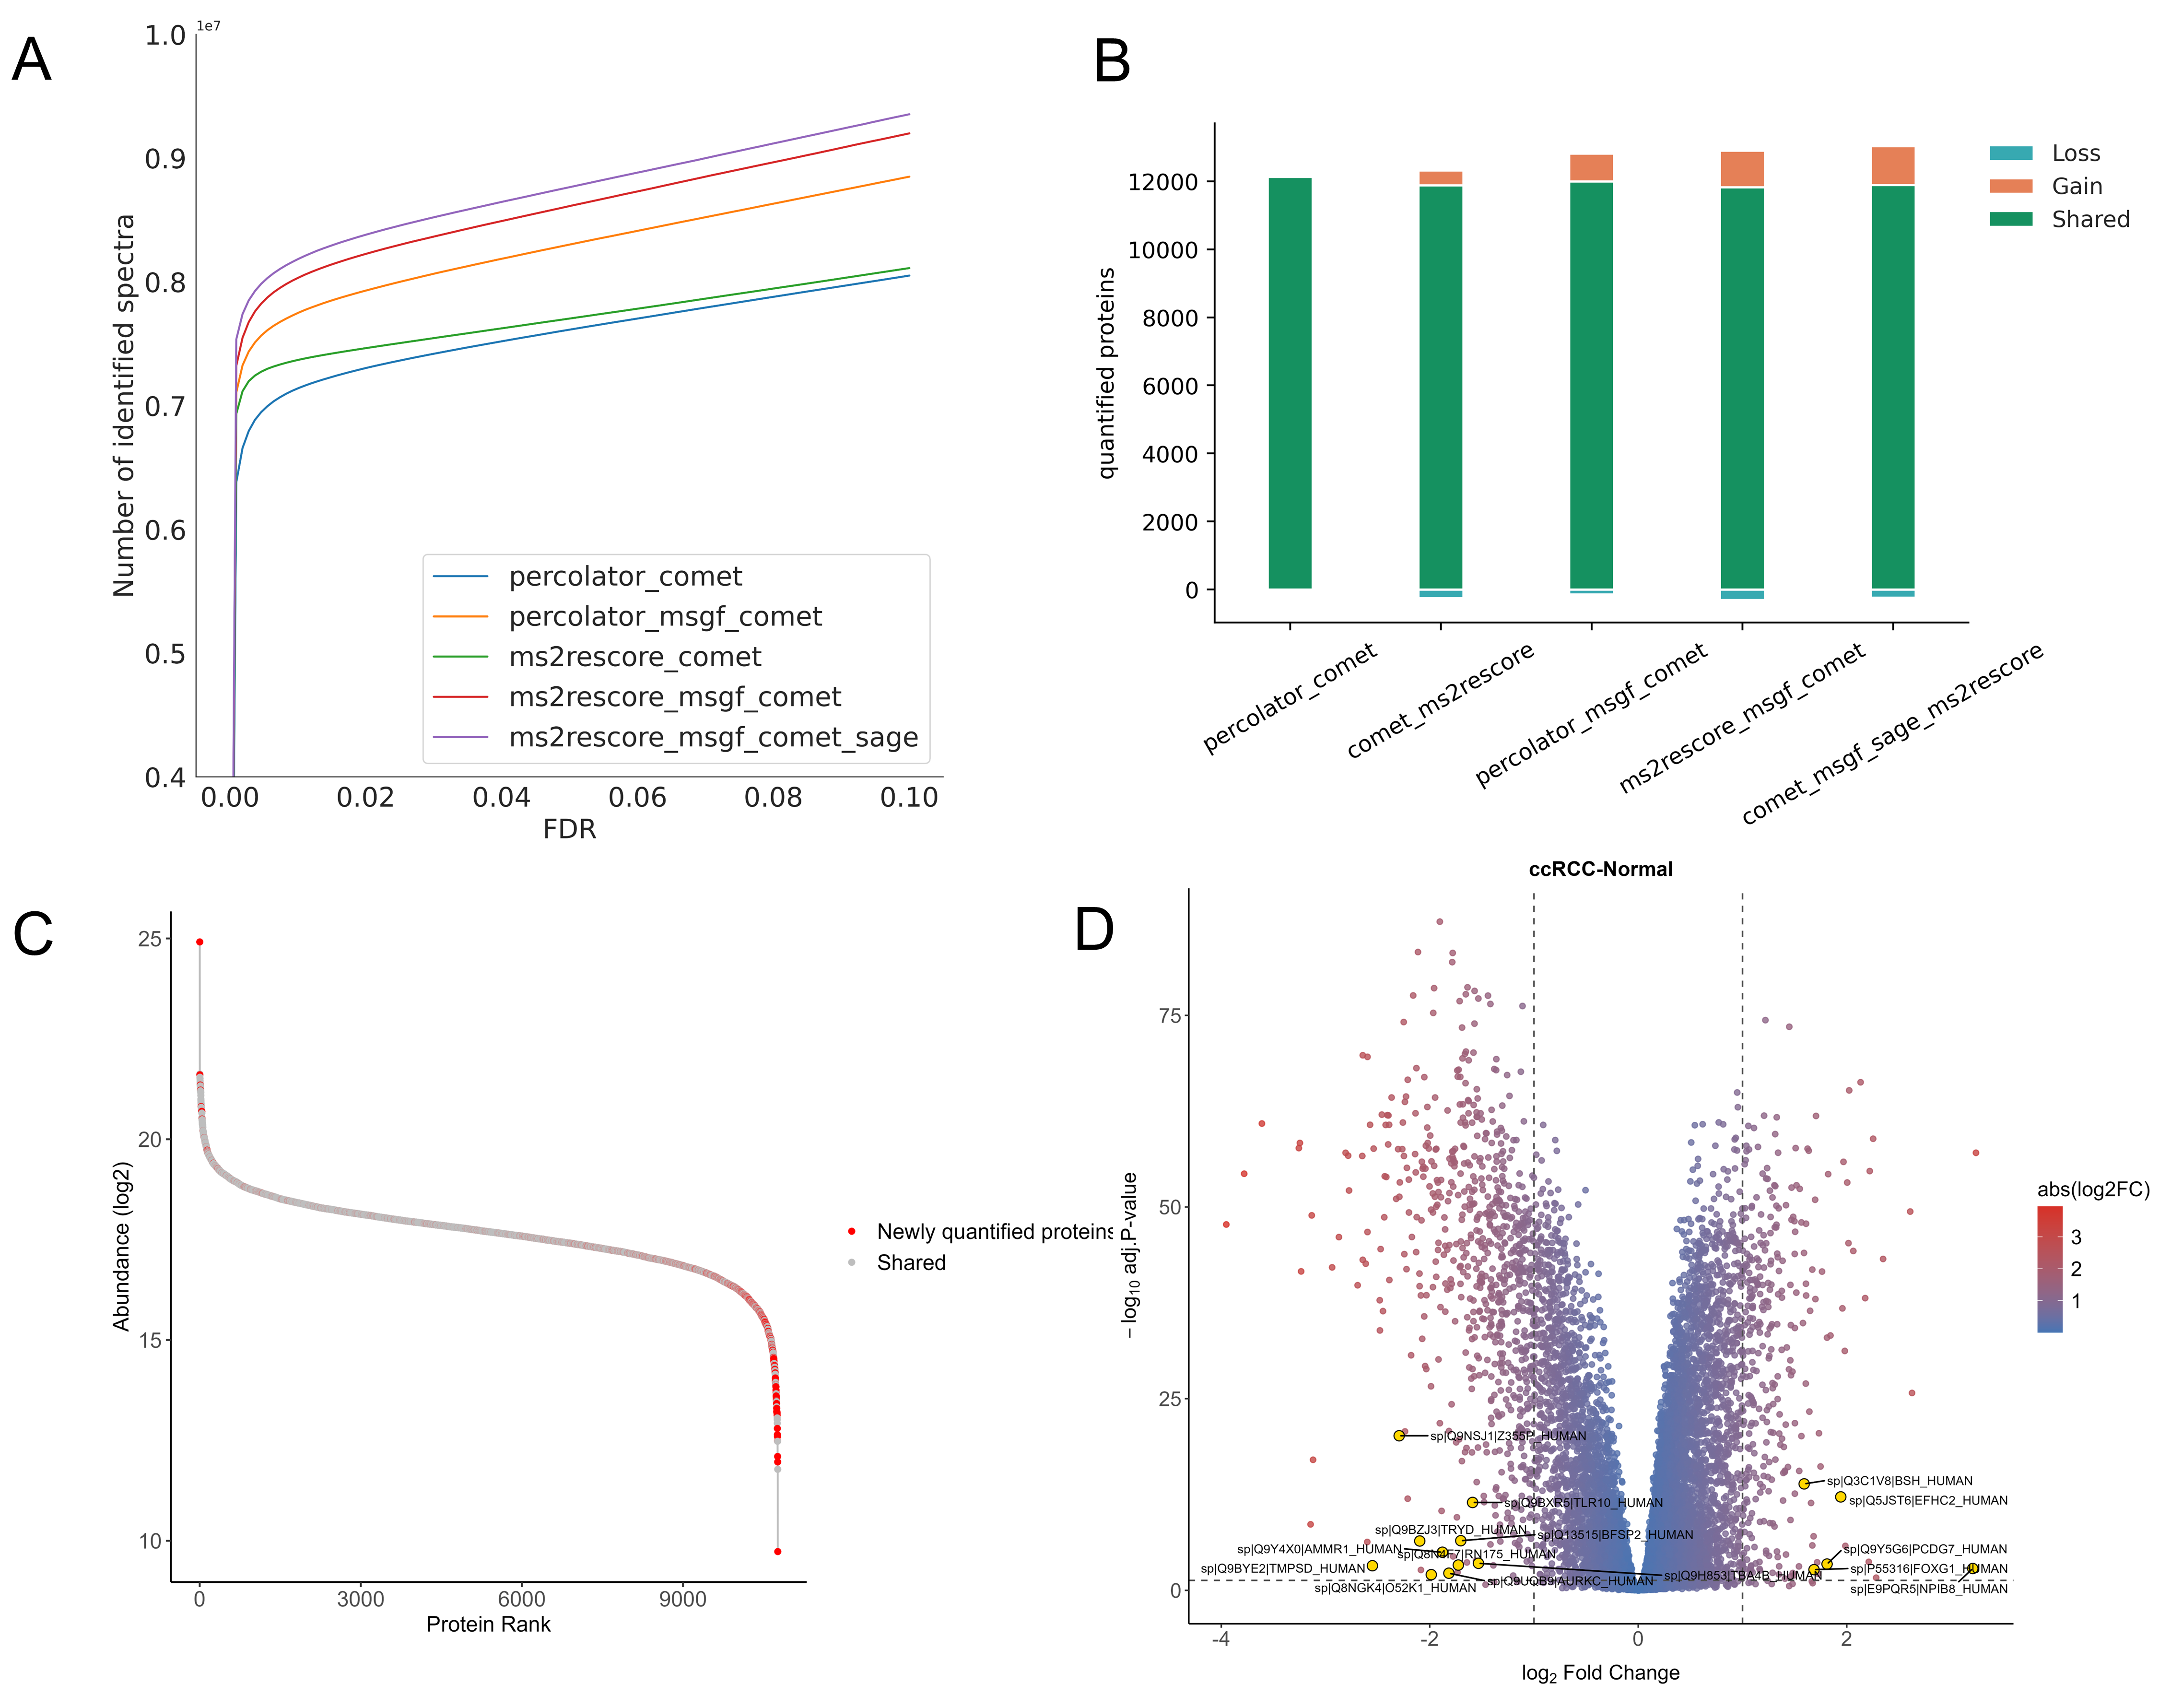
\includegraphics[width=1\textwidth]{figures//CPTAC_TMT.png}
	\caption{Comparison of identification and quantification results for different workflow settings. (A) The number of identified spectra as a function of differing FDR levels for different workflow settings. (B) The number of quantified proteins. The green part indicates the intersection between a workflow and Comet results. (C) The rank of protein abundance from Comet and MSGF+ with MS²Rescore. The red dots represent proteins quantified only in the Comet and MSGF+ with MS²Rescore workflow compared to the Comet and MSGF+ workflow without MS²Rescore. (D) The volcano plot for differential expression analysis from MSstatsTMT. The yellow dots represent proteins quantified only in the Comet and MSGF+ with MS²Rescore workflow compared to the Comet and MSGF+ workflow without MS²Rescore.} % I think you meant yellow dots, but not sure
	\label{fig:PDC_ms2rescore}
\end{figure}

\subsection{quantms with MS²Rescore Improves HLA Class I Immunopeptidome Identification}
To further assess the performance of the quantms workflow using MS²Rescore, we analyzed the HLA Class I immunopeptidomics dataset PXD019643. Five workflow configurations were evaluated: (1) Comet + Percolator, (2) Comet + MS²Rescore, (3) Comet + MSGF+ + Percolator, (4) Comet + MSGF+ + MS²Rescore features, and (5) Comet + MSGF+ + MS²Rescore + SNR features. These configurations were compared based on both the total number of peptide-spectrum matches (PSMs) and the number of unique peptide sequences identified. Across all comparisons, the use of multiple search engines combined with MS²Rescore features significantly enhanced identification performance. At both 1\% and 0.1\% FDR thresholds, integrating MSGF+ with Comet increased the number of identified spectra by 11.7\% compared to using Comet alone. Adding MS²Rescore features on top of the multi-engine workflow yielded a further 22.8\% improvement, as shown in Figure~\ref{fig:PXD019643_immunopeptides}.

To better understand the impact of MS²Rescore-derived features on rescoring, we visualized the distributions of decoy PSMs, rejected target PSMs, and accepted target PSMs using the Pearson correlation coefficient (PCC) and retention time error (Figure 3C, D). The accepted target PSMs were clearly separated from both decoy and rejected targets based solely on PCC values, and exhibited consistently low retention time deviations. These patterns were observed across both individual search engine support and multi-engine consensus, further confirming that the integration of intensity and RT-based features enhances PSM discrimination. Overall, these results demonstrate the robustness of the quantms workflow in immunopeptidomics, highlighting its ability to leverage machine learning-derived features to maximize identification accuracy through multi-engine consensus rescoring.

% Figure Example
\begin{figure}[ht!]
	\centering
	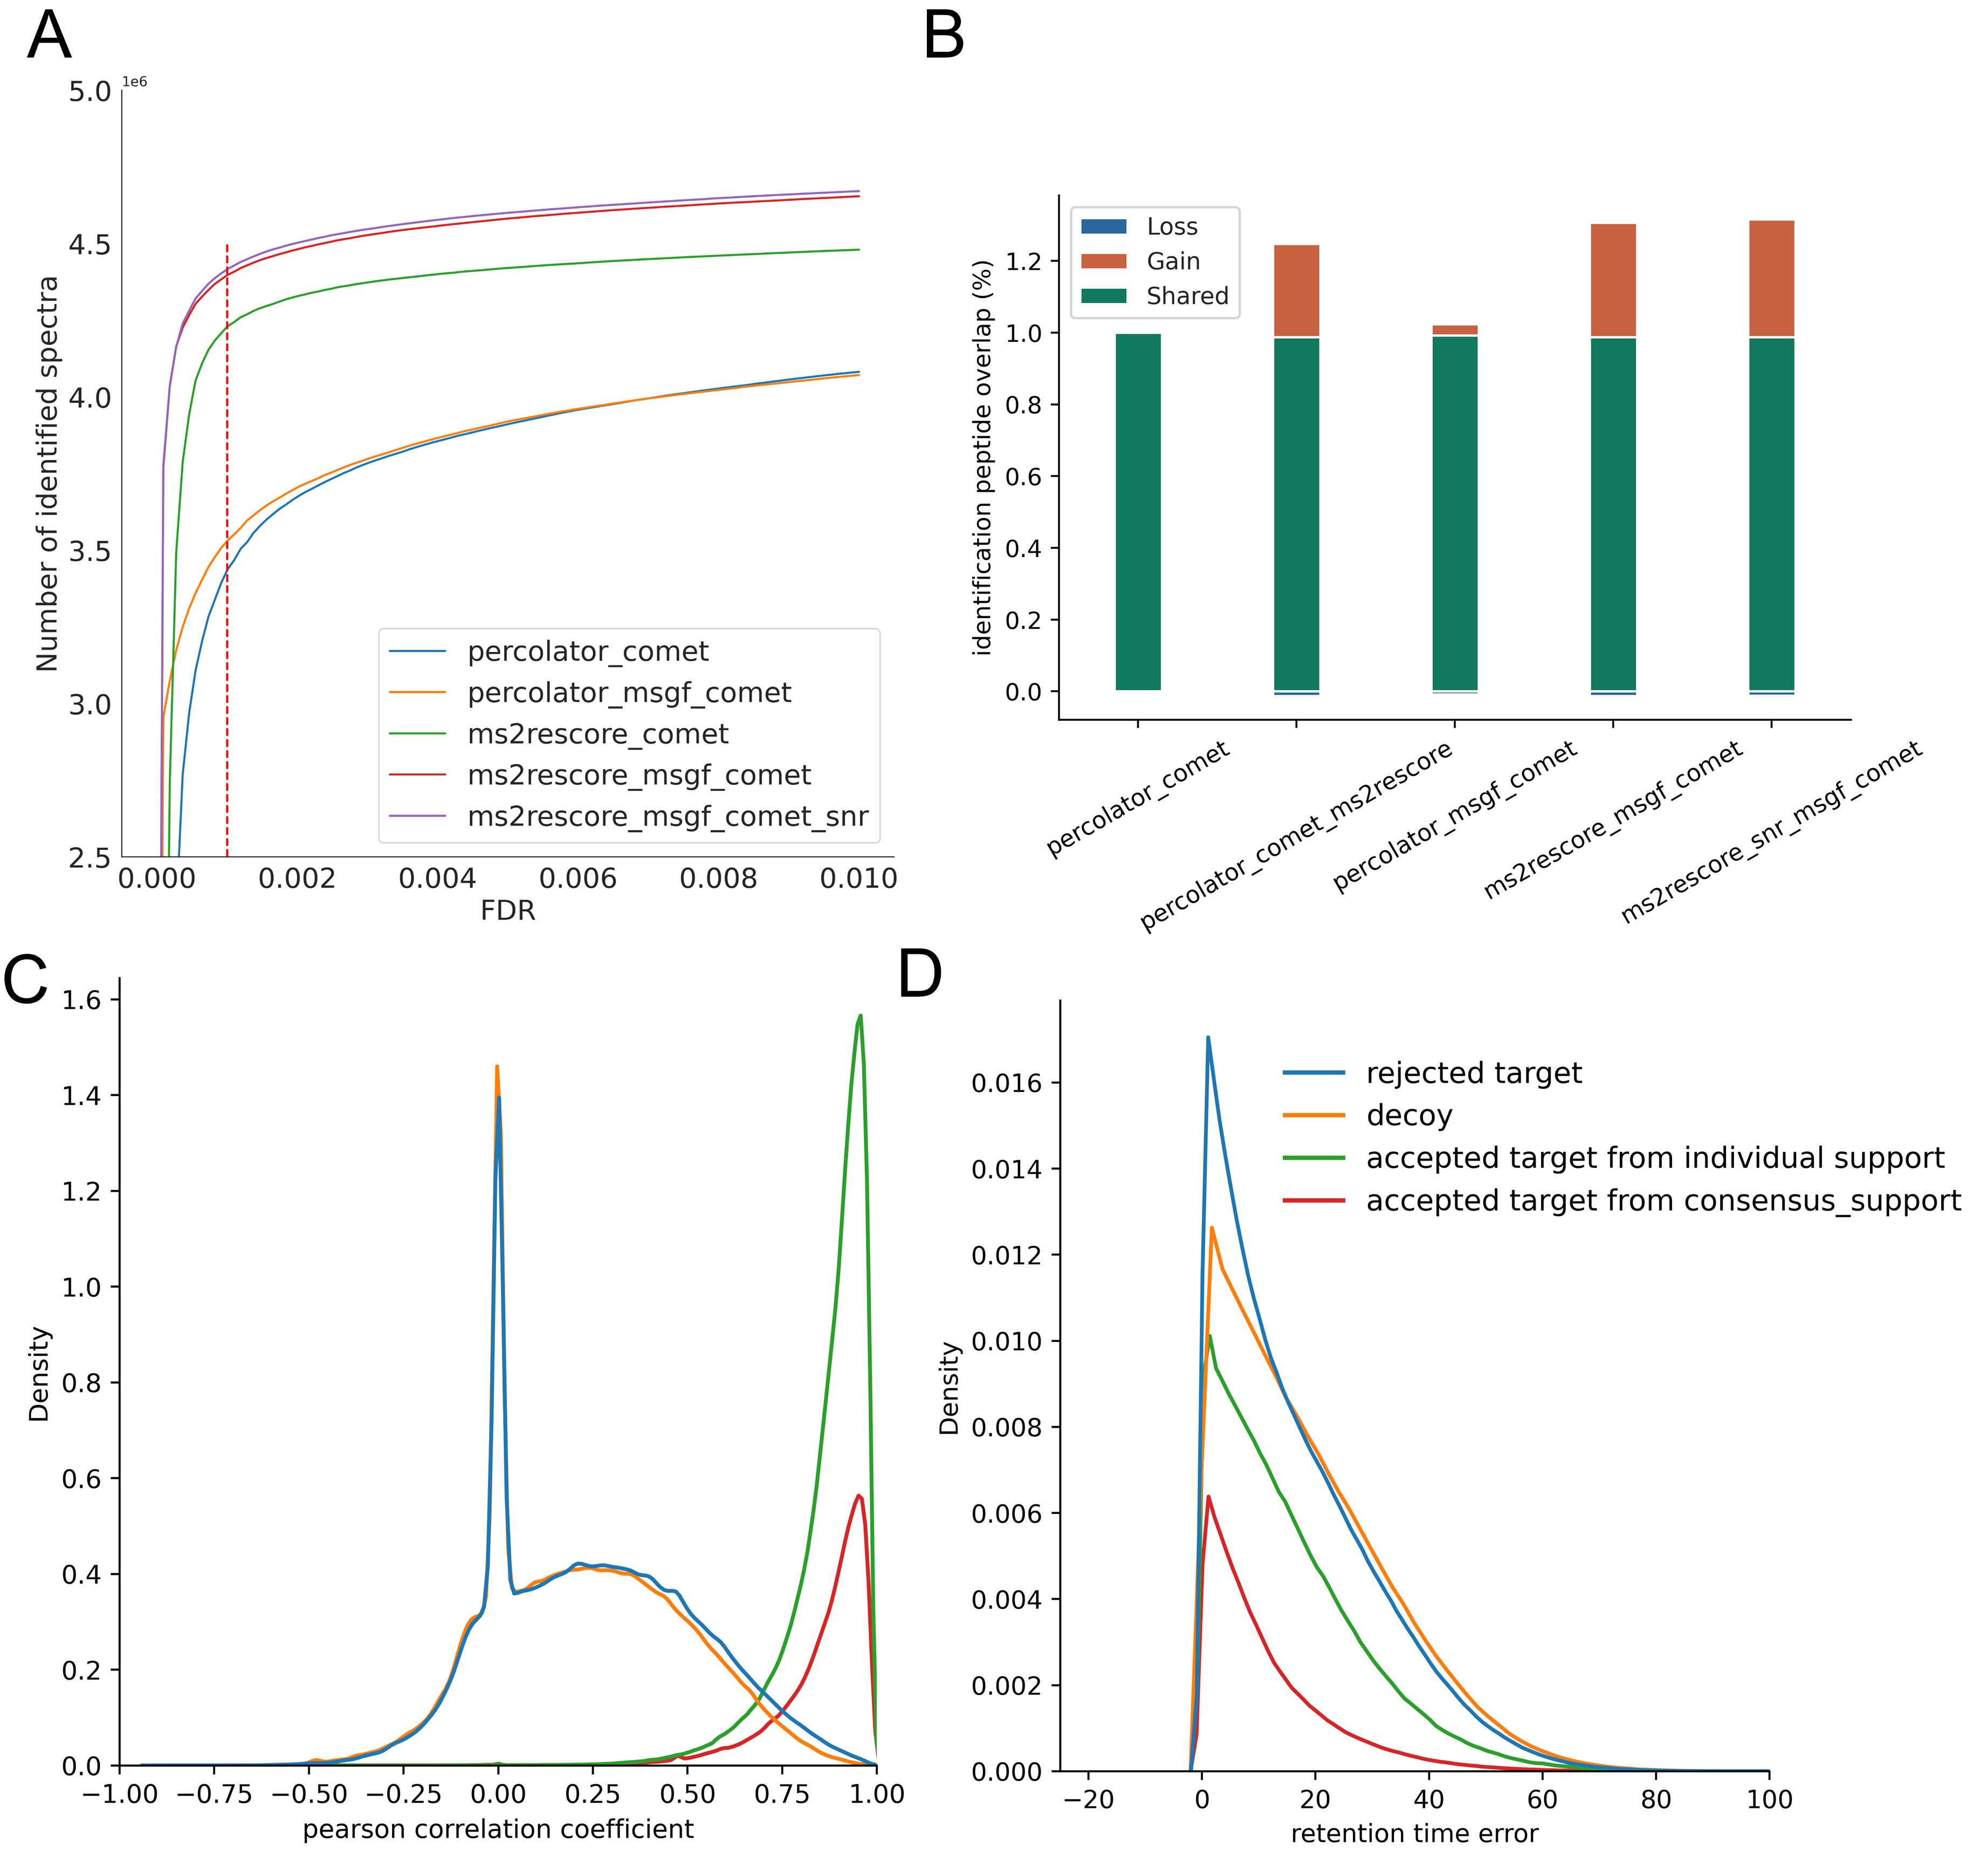
\includegraphics[width=1\textwidth]{figures//PXD019643.png}
	\caption{Comparison of immunopeptides identification results for different workflow settings. (A) Line plot showing the number of spectra identified for four workflow settings at different PSM FDR levels. (B) Percentage of unique identified peptides using different workflow settings. Density plots showing the distribution of the smallest retention time error between observed and predicted retention time (C) and the Pearson correlation between observed and predicted peak intensities (D) for each PSM split into decoys (red), rejected targets with q-value $>$0.01 (blue), and accepted targets from individual support and consensus support with q-value $<$0.01 (green). Note that the rejected targets distribution coincides with the decoy distribution.}
	\label{fig:PXD019643_immunopeptides}
\end{figure}

\subsection{Enhanced Phosphopeptide Identification and Localization Using MS²Rescore integration}
In addition, we investigated the performance of our quantms workflow with MS²Rescore on post-translational modification experiments (PXD026824). For phosphoproteomics analyses, different workflow settings were evaluated: (1) Comet + Percolator, (2) Comet + MS²Rescore, (3) Comet + MSGF+ + Percolator, and (4) Comet + MSGF+ + MS²Rescore features. As shown in Figure~\ref{fig:PXD026824_ms2rescore}, combining search engine consensus results with MS²Rescore features substantially improves Percolator's ability to discriminate between true and false PSMs. This is evident from the leftward shift in score distributions compared to the Comet-only workflow, indicating improved stringency. Additionally, an upward shift in the plot demonstrates a notable gain in the identification rate. Specifically, incorporating MS²Rescore features into the two-search-engine consensus increased the number of identified spectra by 19\% compared to consensus identification alone (Figure 4A). The top 20 feature weights from Percolator, displayed in Supplemental Figure~\ref{fig:phospho_features}, highlight the consistent importance of features such as DotProdIonYNorm, similar to previous datasets.

Given the importance of false localization rate (FLR) control in phosphoproteomics, we also assessed the impact of different workflows on phosphopeptide identification at varying FLR thresholds (Figure 4B, C). At a 0.01 local FLR, the consensus workflow with MS²Rescore features identified 17\% more phosphorylated peptides than its counterpart without MS²Rescore. Notably, 1,345 phosphorylated peptides were uniquely identified by the MS²Rescore-enabled workflow. At the phosphosite level, this workflow also uncovered 350 novel protein phosphorylation sites not reported in the other settings (Figure 4D). Collectively, these results underscore the value of MS²Rescore in enhancing both identification sensitivity and site-level localization in phosphoproteomics, establishing quantms as a robust solution for large-scale PTM data analysis.

% Figure Example
\begin{figure}[ht!]
	\centering
	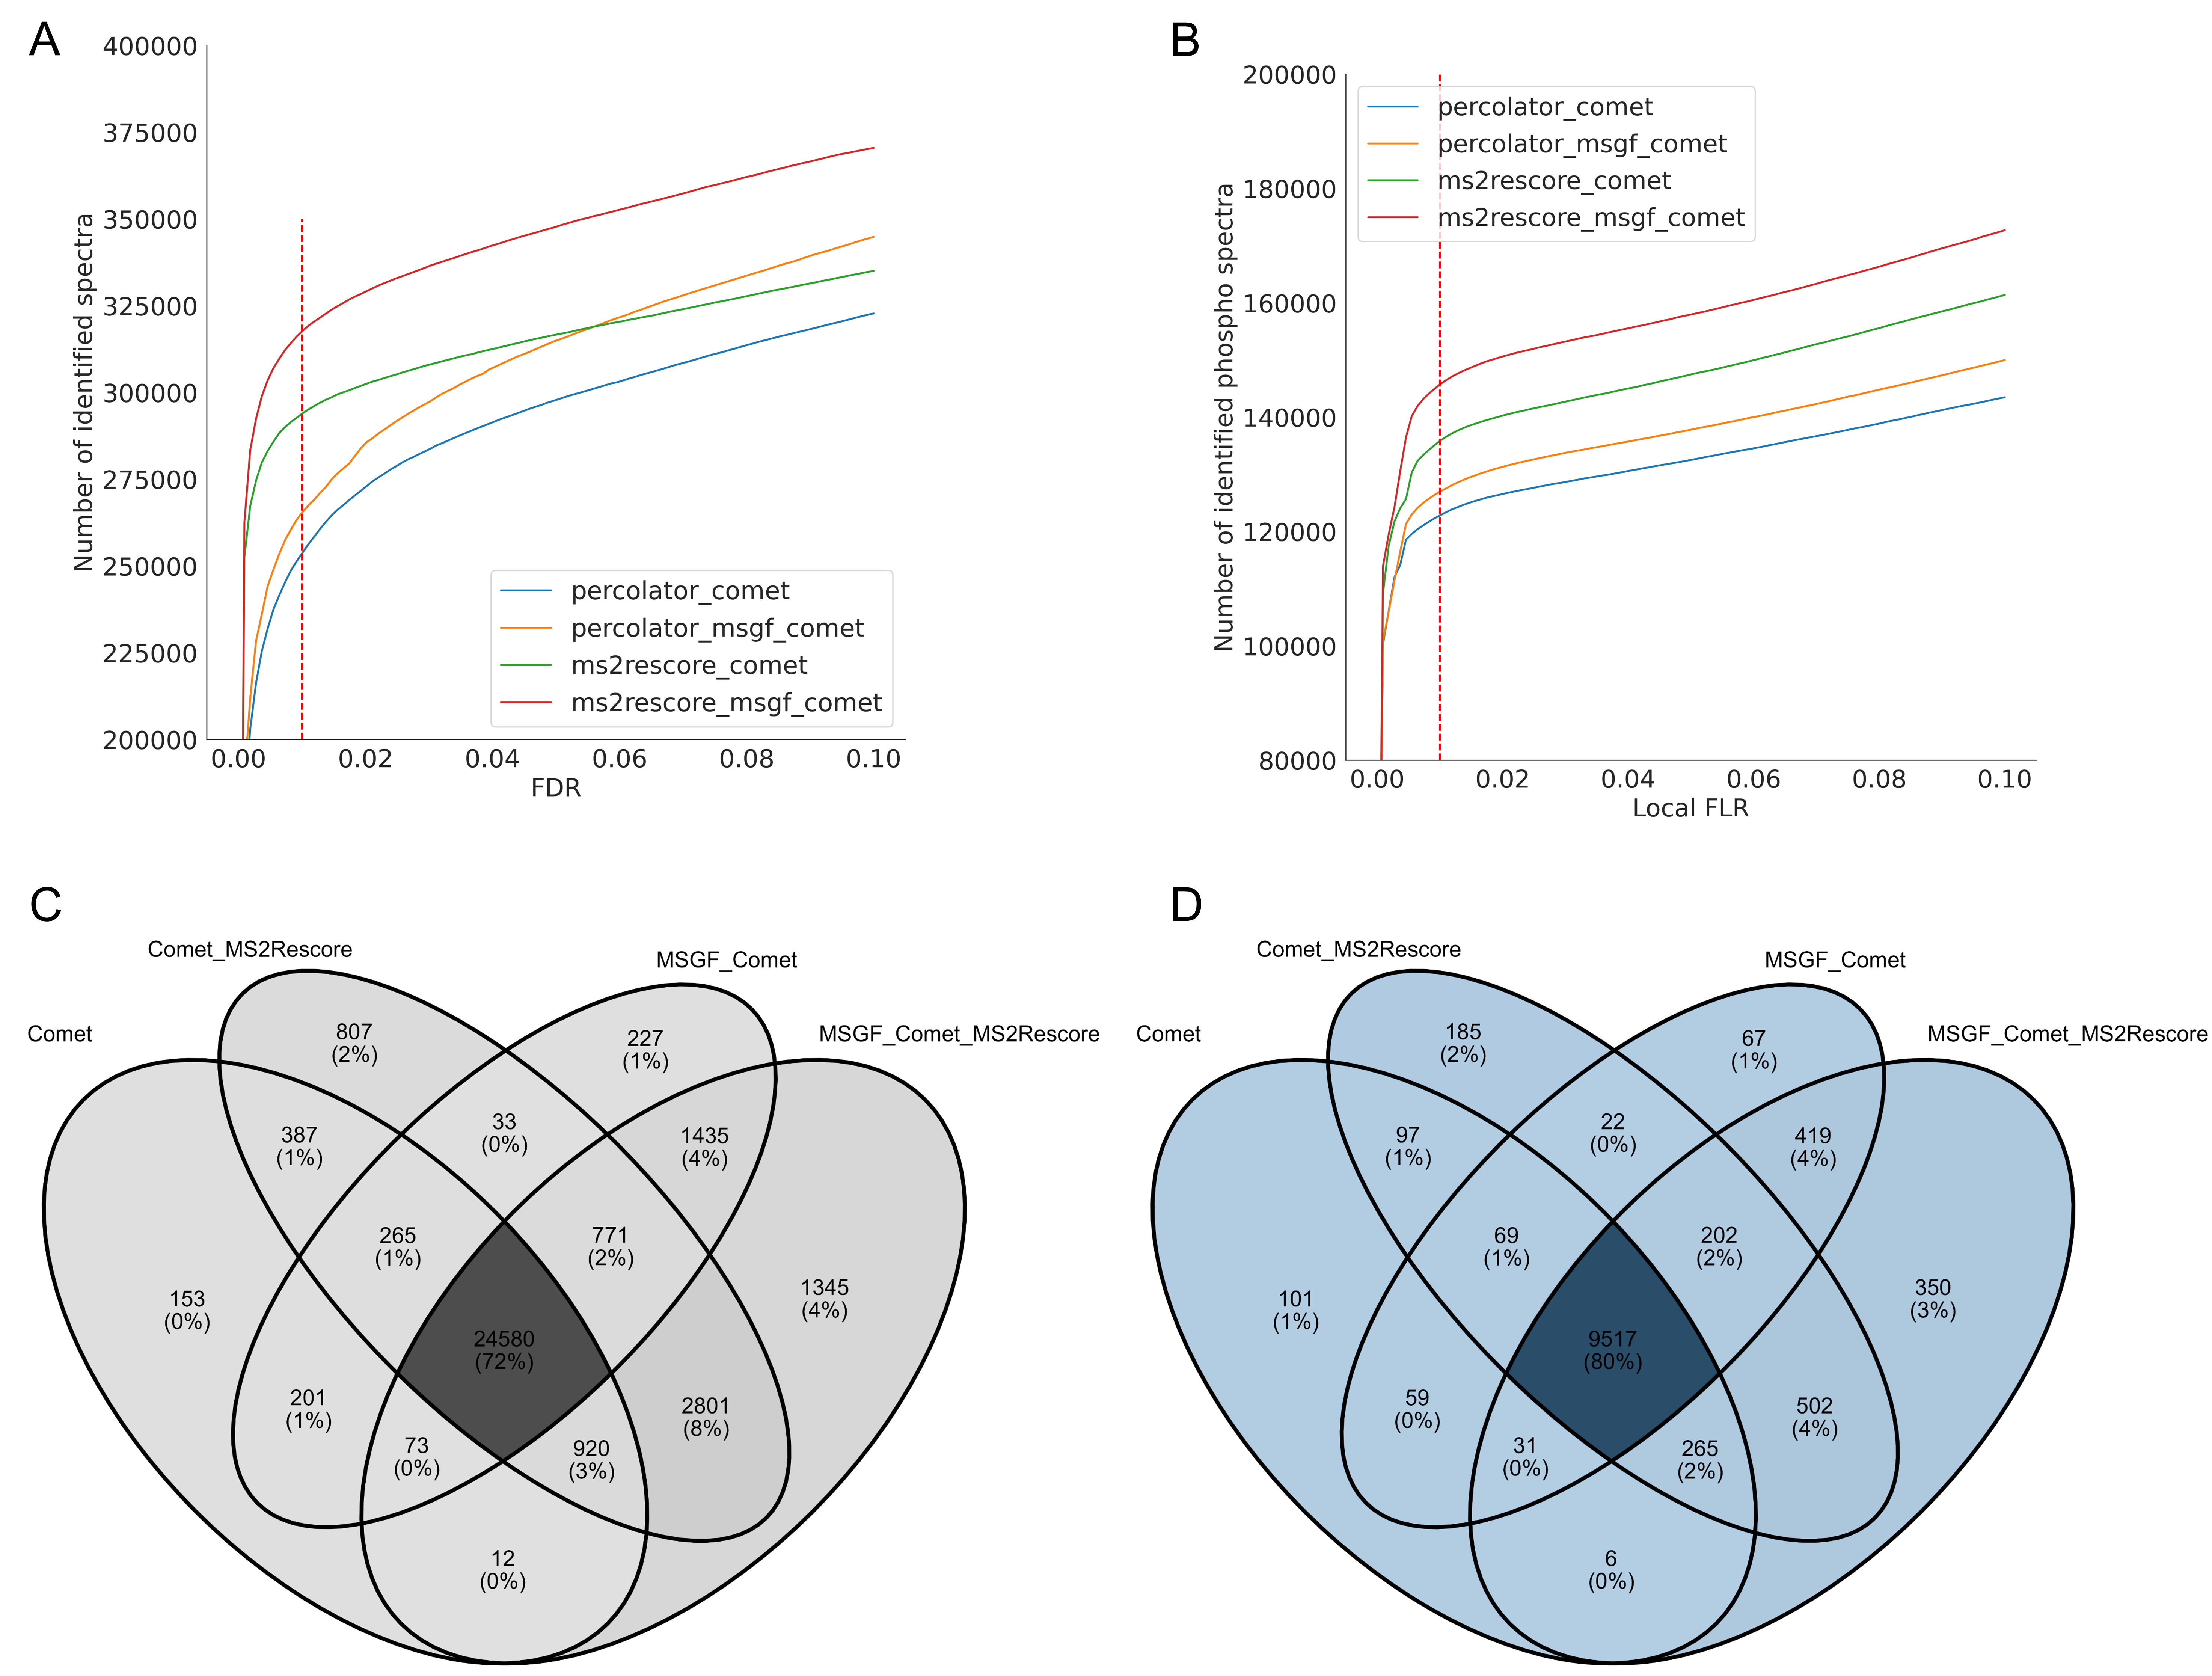
\includegraphics[width=1\textwidth]{figures//phospho2.png}
	\caption{Comparison of phosphorylated peptide identification results for different workflow settings. (A) Line plot showing the number of spectra identified for four workflow settings at different PSM FDR levels. (B) Line plot showing the number of phosphorylated spectra identified for four workflow settings at different local false localization rate levels after an FDR of less than 0.01 at the PSM level. (C) Venn diagram of peptides quantified for four settings. (D) Venn diagram of protein phosphosites at protein FDR 0.01 and FLR 0.01 for four settings.}
	\label{fig:PXD026824_ms2rescore}
\end{figure}

\section{Discussion}
Advancements in deep learning-based tools have significantly improved the accuracy and sensitivity of peptide-spectrum match (PSM) rescoring, yet their integration into streamlined, reproducible, and quantitative proteomics workflows has remained limited, especially for large-scale public data analysis. In this study, we demonstrate the systematic incorporation of MS²Rescore into the open-source quantms pipeline and evaluate its impact across various experimental settings, including label-free quantification (LFQ), tandem mass tag (TMT)-based quantification, immunopeptidomics, and phosphoproteomics. Our results show that enhanced feature sets derived from MS²PIP and DeepLC not only increase the identification rates but also improves the quantification depth. Importantly, we provide evidence that the improved identifications via rescoring propagate downstream into quantification, leading to increased numbers of proteins with reliable abundance estimates, as well as enhanced detection of differentially expressed proteins.

To demonstrate the applicability and advantages of quantms integrated with MS²Rescore in quantitative proteomics, we performed a series of reanalyses using publicly available large-scale datasets with well-established benchmarks. In label-free experiments, MS²Rescore-enhanced workflows achieved significant increases in PSM and peptide identification while maintaining or improving quantification reproducibility across replicates. For TMT experiments, the integration of MS²Rescore into quantms increased the number of quantifiable proteins. In more challenging applications, such as immunopeptidomics and phosphoproteomics, the deep learning-based rescoring pipeline consistently yielded higher identification rates and improved sensitivity. These improvements contribute meaningful biological insights, such as phosphosite discovery and the identification of differentially expressed proteins with potential clinical relevance. In addition, We counted the runtimes with different configurations and it is true that by re-scoring it does add a portion of 15\%-50\% of run-time, as shown as Supplemental Table ~\ref{tab:resources_stats}. This can be alleviated by increasing the number of quantms-rescoring parallel processes. % Maybe add to this sentence that this is especially easy in nextflow. IMHO it does not add a lot

Overall, the results highlight the synergistic benefits of integrating machine learning-based features within end-to-end, cloud-based proteomics workflows. By embedding MS²Rescore into the quantms pipeline, we provide a practical and accessible solution for the community to leverage cutting-edge spectral prediction and retention time modeling without the need for complex manual configuration. This integrated approach enables reproducible reanalysis of large public datasets, increases identification confidence, and strengthens quantitative conclusions across diverse experimental designs. Future work will focus on expanding this approach to other types of post-translational modifications and exploring the integration of additional machine learning tools to further enhance proteomics data analysis capabilities. % I would maybe exclude this last sentence

\section*{Acknowledgments}
We thank all those who supported this research, including funding bodies and the proteomics community for making public datasets available. 
Yasset Perez-Riverol would like to acknowledge funding from EMBL core funding, Wellcome grants (208391/Z/17/Z, 223745/Z/21/Z) and the BBSRC grant ‘DIA-Exchange’ [BB/X001911/1].
R.G., L.M., and R.B. acknowledge funding from [12B7123N,G010023N,G028821N,12A6L24N]. L.M. acknowledge funding from the Horizon Europe Projects BAXERNA 2.0 [101080544] and COMBINE [101191739], and from the Ghent University Concerted Research Action [BOF21/GOA/033]. L.M. is further supported by the CHIST-ERA project ODEEP-EU [G0GDV23N].

% References Section
\bibliographystyle{unsrt}  % Unsorted style for natbib
\bibliography{references}  % references.bib file contains your bibliography


\renewcommand\thefigure{S\arabic{figure}}
\setcounter{figure}{0}

% Figure Example
\begin{figure}[ht!]
	\centering
	\includegraphics[width=1\textwidth]{figures//LFQ_weights.png}
	\caption{The weights that Percolator assigns to different features of the search engine feature vector in MSGF+ (A), Comet (B), and SAGE (C) combined with Percolator settings from PXD001819. The more different from zero a weight is (both positive and negative), the more important that feature is in the final Percolator classification.}
	\label{fig:PXD001819_svm_weights}
\end{figure}

% Figure Example
\begin{figure}[ht!]
	\centering
	\includegraphics[width=1\textwidth]{figures//CPTAC_weights.png}
	\caption{The top 20 normalized weights from Percolator for MSGF+ (A), Comet (B), and SAGE (C) identification results from PDC000125.}
	\label{fig:PDC_ms2rescore_weights}
\end{figure}

\begin{figure}[ht!]
	\centering
	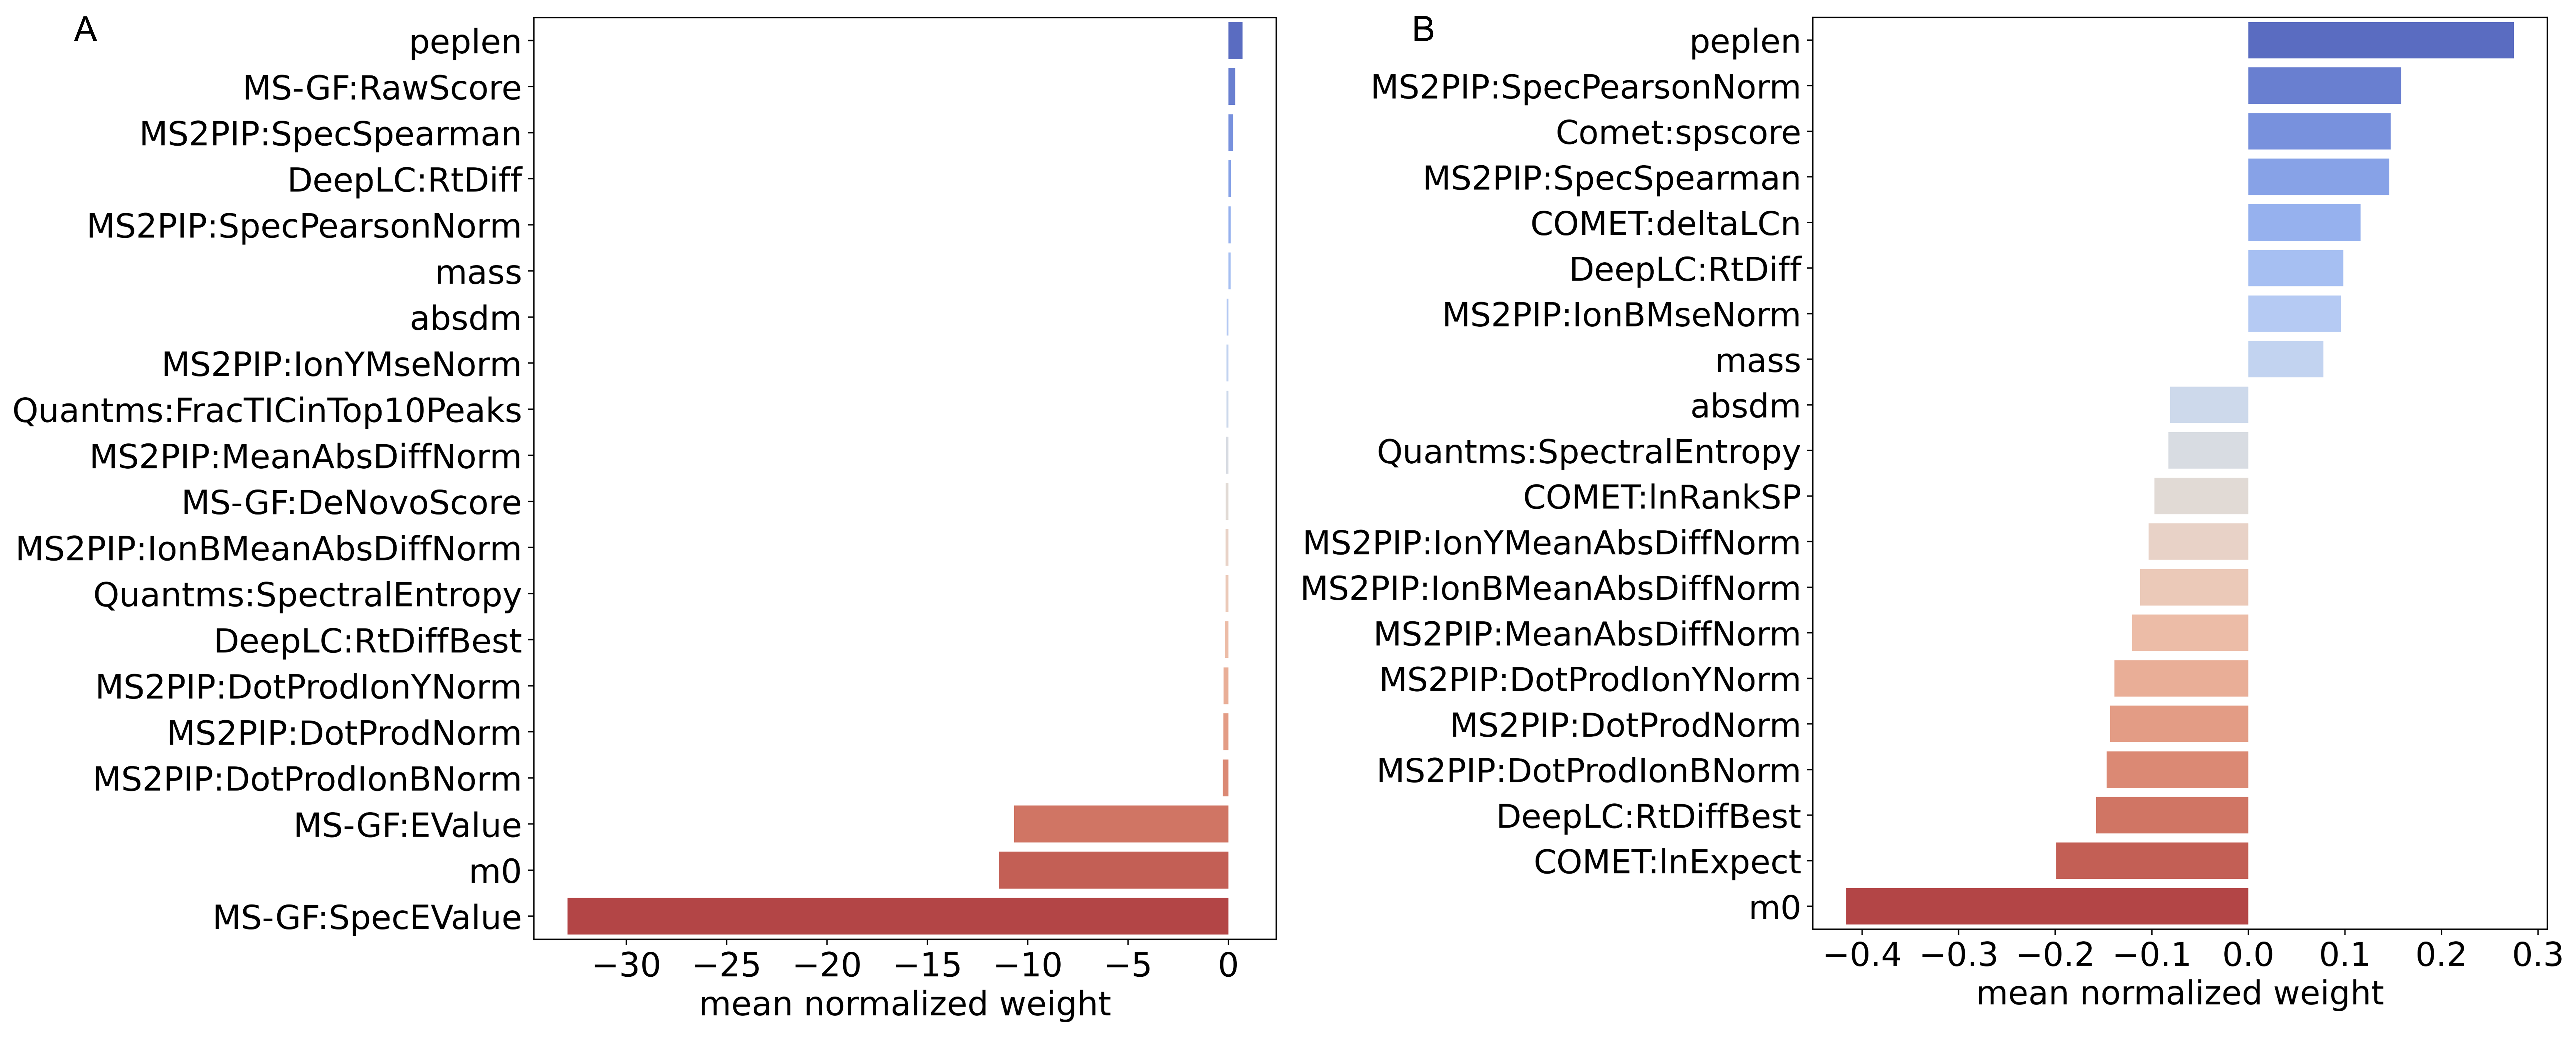
\includegraphics[width=1\textwidth]{figures//PXD019643_weights.png}
	\caption{The top 20 normalized weights from Percolator for MSGF+ (A) and Comet (B) identification results in the PXD019643 dataset.}
	\label{fig:PXD019643_features}
\end{figure}

\begin{figure}[ht!]
	\centering
	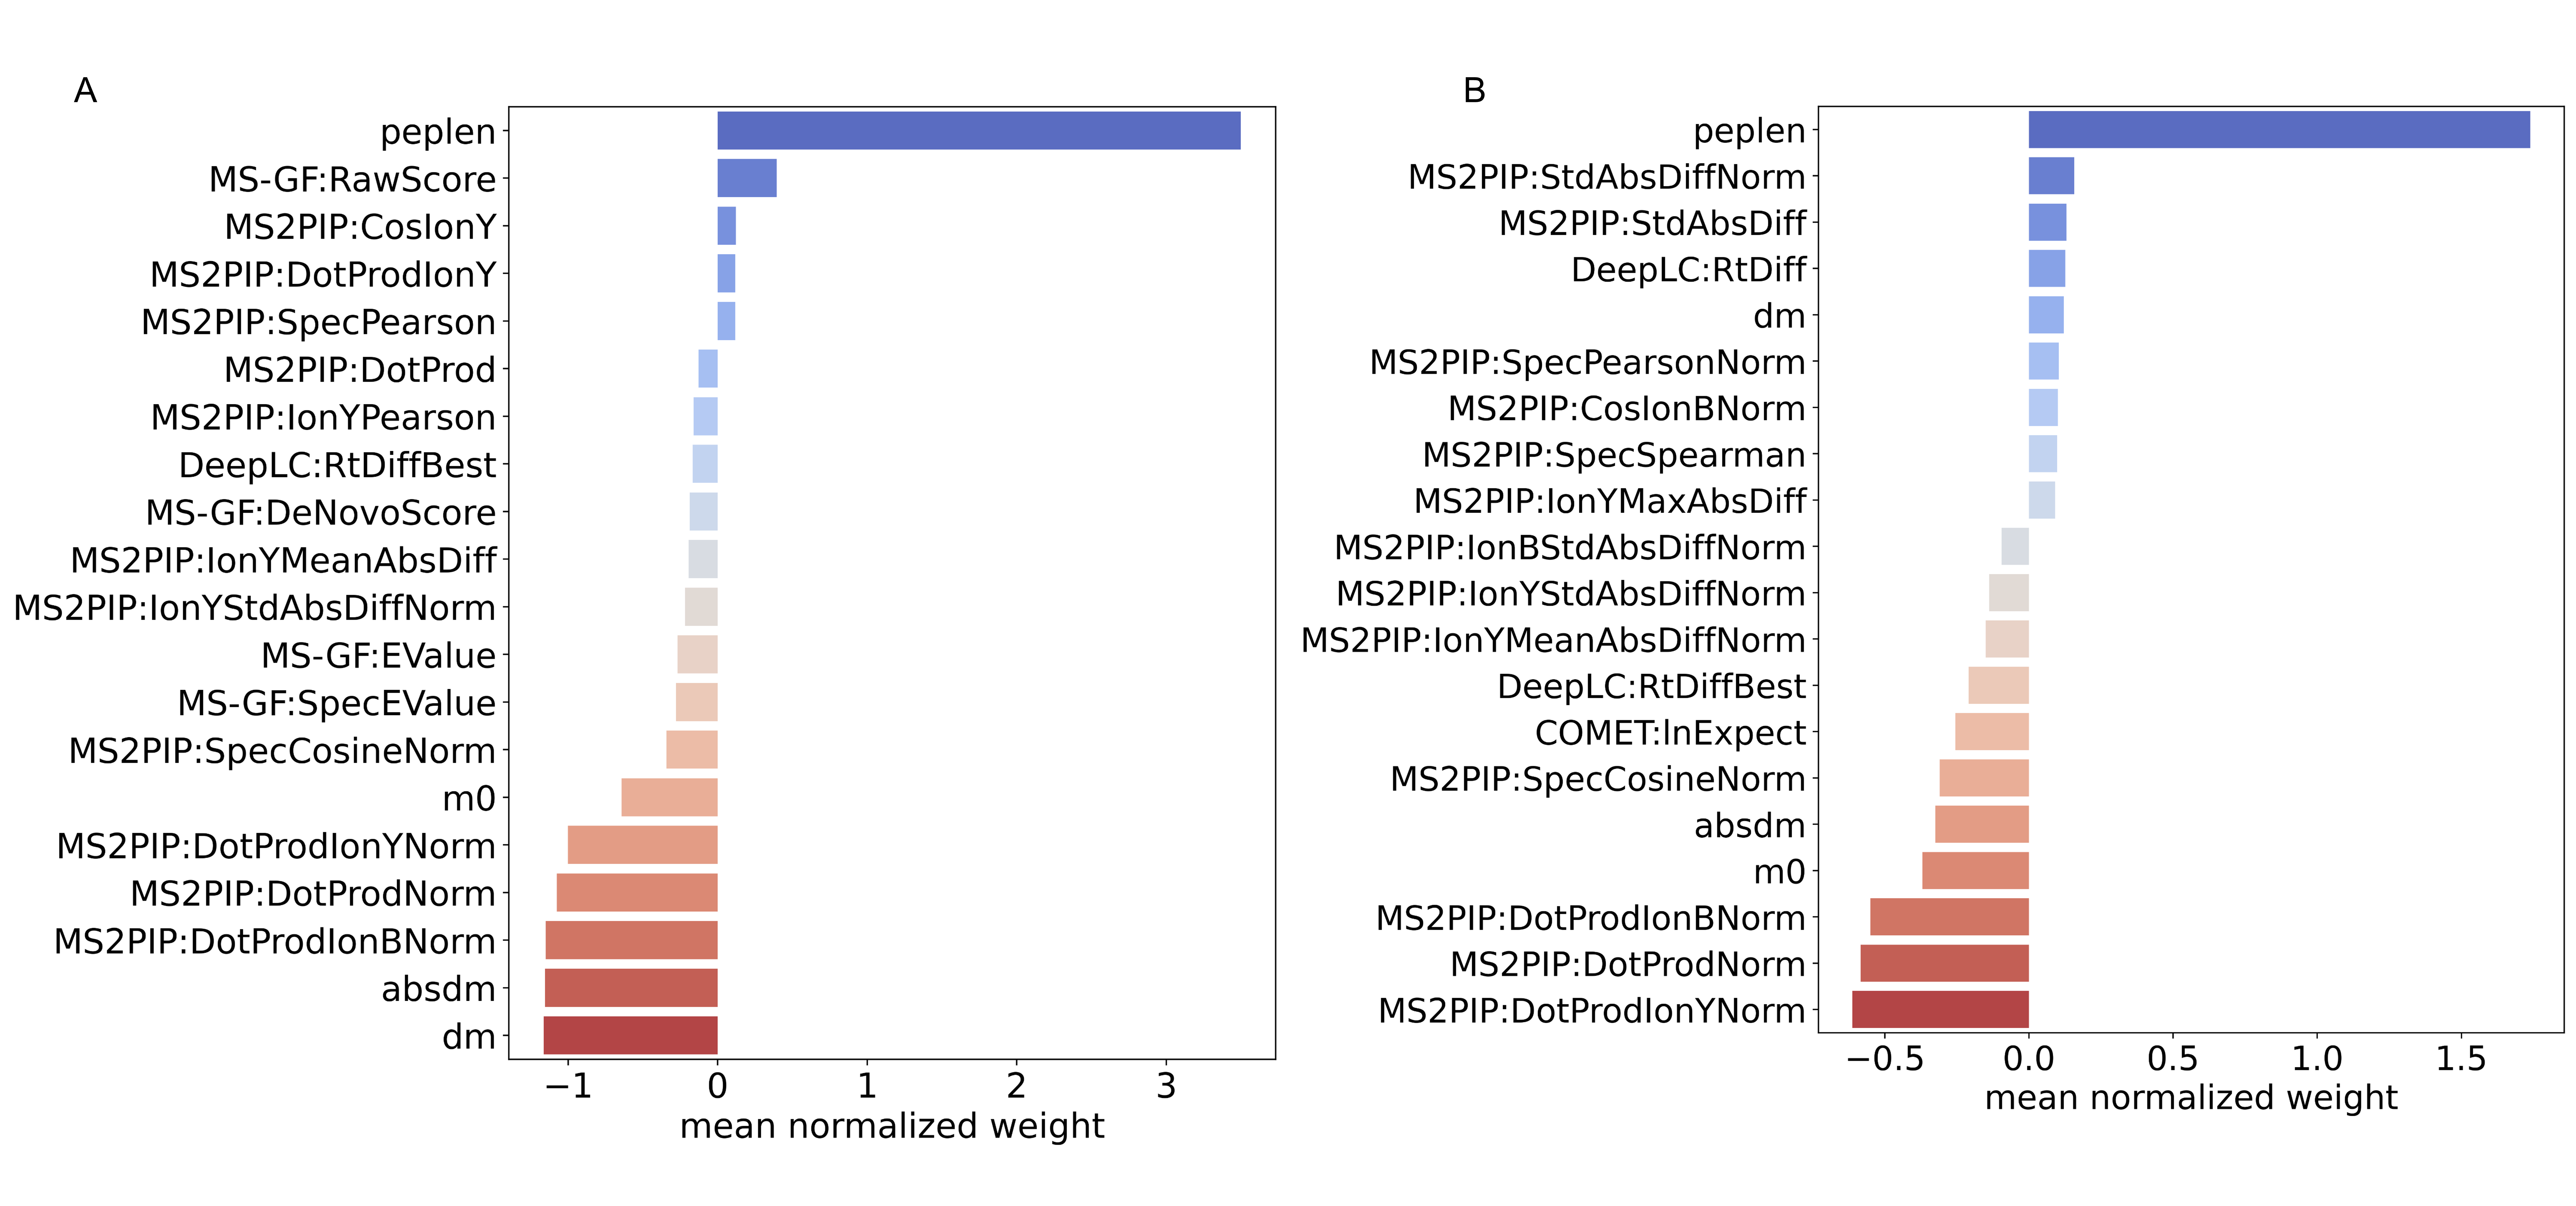
\includegraphics[width=1\textwidth]{figures//phos_weights.png}
	\caption{The top 20 normalized weights from Percolator for MSGF+ (A) and Comet (B) identification results in the PXD026824 dataset.}
	\label{fig:phospho_features}
\end{figure}


\renewcommand\thetable{S\arabic{table}}
\setcounter{table}{0}

% Table Example
\begin{table}[h!]
	\centering
	\caption{Running time, memory and CPU consumption for different Configuration. The memory and CPU values represent the maximum resources required for a single job. The quantms is run in 64 cluster queue.}
	\begin{tabular}{|c|c|c|c|c|}
		\hline
		Datasets & Configuration & Running Time & Memory & CPU \\
		\hline
		PDC000127 & Comet\&MSGF+\&MS²Rescore & 9h39m & 30G & 7 \\
		PDC000127 & Comet\&MSGF+ & 6h28m & 8G & 4 \\
		PDC000127 & Comet & 5h10m & 8G & 4 \\
		PXD019643 & Comet\&MSGF+\&MS²Rescore & 15h57m & 20G & 8 \\
		PXD019643 & Comet\&MSGF+ & 13h09m & 5.5G & 4 \\
		PXD019643 & Comet & 2h05m & 5.5G & 4 \\
		PXD026824 & Comet\&MSGF+\&MS²Rescore & 2h05m & 66G & 8 \\
		PXD026824 & Comet\&MSGF+ & 1h17m & 48.4G & 4 \\
		PXD026824 & Comet & 24m & 48.4G & 4 \\
		\hline
	\end{tabular}
	\label{tab:resources_stats}
\end{table}


\end{document}

